\section{Introduction}

\begin{figure}[t]
    \centering
    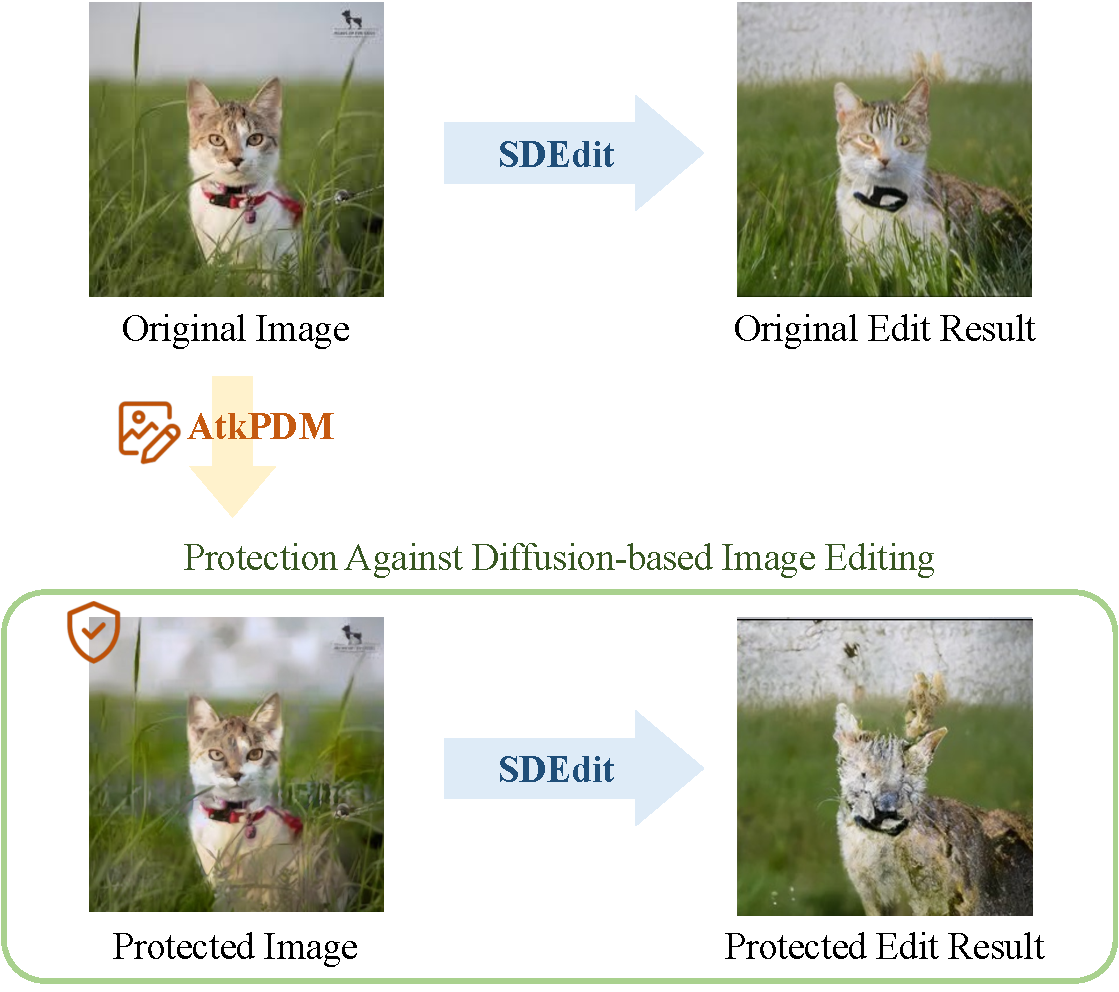
\includegraphics[width=\linewidth]{figures/overview.pdf}
    \caption{Overview of our attack scenario. Diffusion-based image editing can generate high-quality image variation based on the clean input image. However, by adding carefully crafted perturbation to the clean image, the diffusion process will be disrupted, producing a corrupted image or unrelated image semantics to the original image.}
    \label{fig:teaser}
\end{figure}

In recent years, Generative Diffusion Models (GDMs)~\cite{ho2020denoising, song2021denoisingdiffusionimplicitmodels} emerged as powerful generative models that can produce high-quality images, propelling advancements in image editing and artistic creations. The \textit{ease} of using these models to edit~\cite{meng2021sdedit, wang2023stylediffusion, zhang2023inversion} or synthesize new image~\cite{dhariwal2021diffusion, rombach2022high} has raised concerns about potential malicious usage and intellectual property infringement. For example, malicious users could effortlessly craft fake images with someone's identity or mimic the style of a specific artist. An effective protection against these threats is regarded as the diffusion model generating corrupted images or unrelated images to original inputs. Researchers have made significant strides in crafting imperceptible adversarial perturbation on images to safeguard them from being edited by diffusion-based models. 

Previous works such as PhotoGuard~\cite{salman2023raisingcostmaliciousaipowered} and Glaze~\cite{shan2023glazeprotectingartistsstyle} have effectively attacked Latent Diffusion Models (LDMs) by minimizing the latent distance between the protected images and their target counterparts. PhotoGuard first introduce attacking either encoders or diffusion process in LDMs via Projected Gradient Descent (PGD)~\cite{madry2018towards} for the protection purpose; however, it requires backpropagating the entire diffusion process, making it prohibitively expensive. Subsequent works AdvDM~\cite{liang2023adversarialexampledoesgood} and Mist~\cite{liang2023mistimprovedadversarialexamples} leverage the semantic loss and textural loss combined with Monte Carlo method to craft adversarial images both effectively and efficiently. Diff-Protect ~\cite{xue2024diffusion} 
further improve adversarial effectiveness and optimization speed via Score Distillation Sampling (SDS) ~\cite{poole2022dreamfusiontextto3dusing2d}, setting the state-of-the-art performance on LDMs.

However, previous works primarily focus on LDMs, and attacks on Pixel-domain Diffusion Models (PDMs) remain largely unexplored. Xue et al. ~\cite{xue2024diffusion} also highlighted a critical limitation of current methods: the attacking effectiveness is mainly attributed to the vulnerability of the VAE encoders in LDM; however, PDMs don't have such encoders, making current methods hard to transfer to PDMs. The latest work \cite{xue2024pixelbarrierdiffusionmodels} has attempted to attack PDMs, but the result suggests that PDMs are robust to pixel-domain perturbations. Our goal is to mitigate the gap between these limitations.

In this paper, we propose an innovative framework designed to effectively attack PDMs. Our approach includes a novel \textbf{feature attacking loss} that exploits the vulnerabilities in denoising UNet to distract the model from recognizing the correct semantics of the image, a \textbf{fidelity loss} that acts as optimization constraints that ensure the imperceptibility of adversarial image and controls the attack budget, and a \textbf{latent optimization strategy} utilizing victim-model-agnostic VAEs to further enhance the naturalness of our adversarial image closer to the original. With extensive experiments on different PDMs, the results show that our method is effective and affordable while robust to traditional defense methods and exhibiting attack transferability in the black-box setting. 

In addition, our approach outperforms current semantic-loss-based and PGD-based methods, reaching state-of-the-art performance on attacking PDMs. Our contributions are summarized as follows:

\begin{enumerate}
    \item We propose a novel attack framework targeting PDMs
    , achieving state-of-the-art performance in safeguarding images from being edited by SDEdit.
    \item  We propose a novel feature attacking loss design to distract UNet feature representation effectively.
    \item We propose a latent optimization strategy via model-agnostic VAEs to enhance the naturalness of our adversarial images.
\end{enumerate}
